\setAuthor{Markus Rene Pae}
\setRound{piirkonnavoor}
\setYear{2021}
\setNumber{G 1}
\setDifficulty{1}
\setTopic{TODO}

\prob{Kuul sfääris}
Kausis, mille sisekülje pinnaks on poolsfäär raadiusega $R=\SI{50}{\centi\meter}$, veereb ühtlase kiirusega mööda horisontaaltasapinnalist ringjoont kuulike. Kuuli tiirlemistasandi kõrgus kausi põhjast on $h=\SI{10}{\centi\meter}$. Leidke kuuli tiirlemisperiood. Eeldage, et kuuli läbimõõt on kausi raadiusega võrreldes tühine ning hõõrdetegur kuuli ning kausi vahel on samuti tühiselt väike. Gravitatsioonikiirendus on $g=\SI{9.8}{\meter\per\second\squared}$.


\hint

\solu
Läheme pöörlevasse taustsüsteemi. Siis mõjub kuulile kolm jõudu, raskusjõud, tsentrifugaaljõud ja toereaktsioon. Nende jõudude summa peab olema 0, sest pöörlevas taustsüsteemis seisab kuulike paigal. Sfääri pinna ja kuuli vahel puudub hõõrdejõud, seega on kuuli raskusjõu ning tsentrifugaaljõu summavektor sfääri raadiuse sihiline~\pp{1}.\par
Olgu $r$ kuulikese kaugus pöörlemisteljest. Sarnaste kolmnurkade tõttu, suhtuvad raskusjõu ja tsentrifugaaljõu teineteisesse kui $R-h$ ja $r$~\pp{1}. Seega peab kehtima seos:
$$ \frac{mg}{R-h} = \frac{m \omega^2 r}{r} \quad \pp2$$
kus $\omega$ on kuulikese ringsagedus. Viimase avaldise lihtsustamine ning sellest nurkkiiruse $\omega$ avaldamine annab:
$$ \omega = \sqrt{\frac{g}{R-h}} \quad \pp2$$
Kuna $\omega = \frac{2\pi}{T}$ \pp{1}, siis järelikult peab tiirlemise periood olema $T = 2 \pi \sqrt{\frac{R-h}{g}} \approx \SI{1.28}{\second}$ \pp{1}.

\begin{figure}[H]
	\centering
	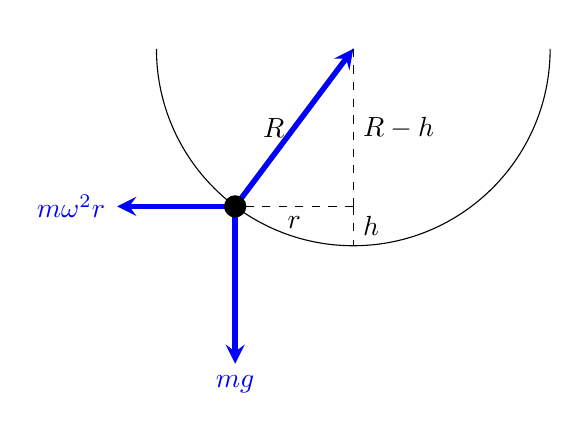
\begin{tikzpicture}[scale=0.5]
    \coordinate (A) at (-5,0);
    \coordinate (O) at (0,0);
    \coordinate (kuul) at (-3,-4);
    \coordinate (base) at (0,-5);
    \coordinate (X) at (0,-4);

    % kauss
    \draw (A) arc (0:180:-5);

    % jooned
    \draw [dashed] (O) -- (0,-4) node[midway,right] {$R-h$};
    \draw (O) -- (-3,-4) node[midway,above,left] {$R$};
    \draw [dashed] (0,-4) -- (base) node[midway,right] {$h$};
    \draw [dashed] (O) -- (kuul);
    \draw [dashed] (X) -- (kuul) node[midway,below] {$r$};

    % jõud
    \draw[line width=2pt,blue,-stealth](kuul)--(-3,-8) node[anchor=north]{$mg$};
    \draw[line width=2pt,blue,-stealth](kuul)--(-6,-4) node[anchor=east]{$m\omega^2r$};
    \draw[line width=2pt,blue,-stealth](kuul)--(O) node[anchor=south west]{};

    % kuul
    \node[circle,fill=black,inner sep=1mm] at (kuul) {};
  \end{tikzpicture}
\end{figure}
\probend